\begin{figure}[!htbp]
  \centering
  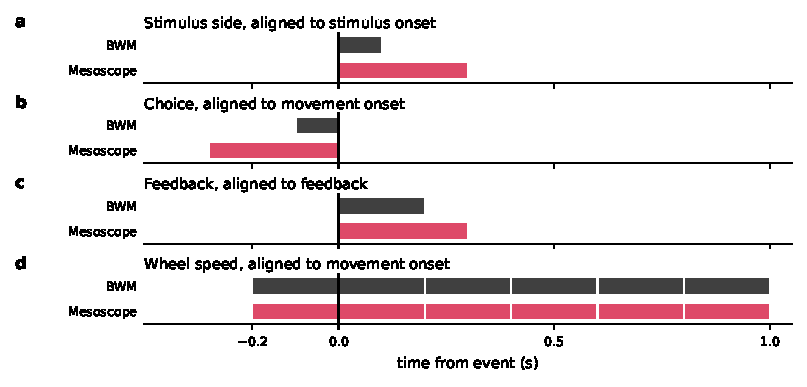
\includegraphics[width=5.35in,height=0.8\textheight,keepaspectratio]{figures/windows.pdf}
  \caption{Analysis windows used for decoding and for the single-neuron tuning test. BWM windows follow the Brain Wide Map single-cell analyses. Mesoscope frames are about 0.2\,s apart, so the mesoscope stimulus, choice and feedback windows are widened to 0.3\,s to always contain at least one frame; the mesoscope value is the mean of the deconvolved trace, linearly interpolated at each neuron's own sampling times, over the window. BWM values are firing rates (spike count / window length). \textbf{a} Stimulus side: activity in window $[0, 0.1]$\,s (BWM) or $[0, 0.3]$\,s (mesoscope) relative to stimulus onset. \textbf{b} Choice: window $[-0.1, 0]$\,s (BWM) or $[-0.3, 0]$\,s (mesoscope) relative to movement onset. \textbf{c} Feedback: window $[0, 0.2]$\,s (BWM) or $[0, 0.3]$\,s (mesoscope) relative to feedback. \textbf{d} Wheel speed: six 0.2\,s bins from $-0.2$ to $1$\,s around movement onset, identical for both modalities; each bin's activity is paired with the mean absolute wheel velocity in the same bin.}
  \label{fig:windows}
\end{figure}
